\documentclass[12pt]{article}
\usepackage{tikz}
\usepackage{bm}
\usepackage{amsmath,amssymb}
\usepackage{textcomp}
\usepackage{listings}
\usepackage[colorlinks=true,pagebackref,linkcolor=blue]{hyperref}
\textwidth=7in
\textheight=9.5in
\topmargin=-1in
\headheight=0in
\headsep=.5in
\hoffset=-.85in


\lstset{
basicstyle=\footnotesize\ttfamily,
language=R,
upquote=true,
breakatwhitespace=true,
columns=fullflexible,
keepspaces,
numbers=none,
tabsize=3,
frame=b,
framextopmargin=20pt,
showstringspaces=false,
extendedchars=true
}

\pagestyle{empty}

\renewcommand{\thefootnote}{\fnsymbol{footnote}}

\usepackage{Sweave}
\begin{document}
\Sconcordance{concordance:jho19HW3.tex:jho19HW3.Rnw:%
1 34 1 1 0 89 1 1 3 17 1 1 5 6 1 4 0 1 3 8 1 4 0 1 3 4 1 4 0 1 3 31 1 1 %
2 9 0 1 6 10 1 1 4 73 1}




\begin{center}
{\bf AMS 550.400 \qquad Homework 3 Additional Instruction \qquad  Due Date: Nov 19}\\
\vskip.2in
{\footnotesize Last Compiled on \today}
\end{center}

\setlength{\unitlength}{1in}

\begin{picture}(6,.1) 
\put(0,0) {\line(1,0){6.25}}         
\end{picture}

\renewcommand{\arraystretch}{2}

\begin{center}
    {\bf General Instruction}
\end{center}
\begin{itemize}
    \item failure to follow the instruction will result in severe penalty
        (graded at 90\% or even worse)
    \begin{itemize}
        \item no second grading is planned for this homework set 
        \item type up your own homework (i.e., no copy-and-pasting from others
            \& you know one can easily check this)
    \end{itemize}
    \item from the home directory \verb+~/+, make a directory for this homework set
        \begin{itemize}
            \item use \verb+mkdir nhleeHW3.git+ for the directory name
            \item create a Sweave file called \verb+nhleeHW3.Rnw+ 
            \item replace \verb+nhlee+ with the ``left-hand side'' of your school email
        \end{itemize}
    \item initialize it as a git folder 
        \begin{itemize}
            \item do this from inside of the git folder for your own sake
            \item make sure to verify that your folder contains a hidden folder called \verb+.git+
            \item set it up from RStudio as a RStudio project with git support
            \item look for \verb+[COMMIT]+ from the text below for the location where you are supposed to add \& commit 
        \end{itemize}
    \item using RStudio for editing and compiling your Rnw file is highly
        recommended 
        \begin{itemize}
            \item to compile, find and press ``Complie PDF'' button within the
                RStudio editor window (typically, the upper left corner window)
            \item alternatively, you can use \verb+R CMD <Sweave/pdflatex>+ from bash-shell
                command line provided that you are in the ``appropriate'' directory
                \begin{lstlisting}
R CMD Sweave yourfilename.Rnw
R CMD pdflatex yourfilename.tex
                \end{lstlisting}
        \end{itemize}

    \item use the \verb+homeworkset3.tex+ file as a starting point for
        typesetting your homework solution
        \begin{itemize}
            \item find it from the course git folder
            \item do not delete the problem statements 
            \item do not delete/modify the existing codes in the preamble area 
        \end{itemize}
    \item once completed, compress the folder as a \verb+.nhleeHW3.zip+ or
        \verb+nhleeHW3.tar.gz+, where \verb+nhlee+ is replaced with one from your school email 
        \begin{itemize}
            \item make sure that your compressed file can actually be decompressed
        \end{itemize}
    \item on the due date, 
        \begin{itemize}
            \item submit a paper copy to the instructor during the class
            \item upload the compressed folder to the designated BB discussion
                forum before midnight
            \item any commit made after the class meeting time will be
                discarded using \verb+git reset --hard+, and will not be
                counted as a part of your homework submission
        \end{itemize}
\end{itemize}

\vskip0.25in
\begin{center}
    \textbf{Problems from Chapter 7: Matrix Algebra for MDS}
\end{center}
\paragraph{Ex 7.18}
\begin{itemize}
    \item[(a)] \verb+[COMMIT]+ Use Sweave to accomplish this
        \begin{itemize}
            \item Use 
\begin{lstlisting}
\includegraphics{jho19HW3-001}
\end{lstlisting}
            \item Make sure to label the horizontal axis, the vertical axis
                and give the main title, and give different color for $A$ and
                $B$ e.g., by filling out the space
                between the quotation marks, and choose a different symbol for
                $A$ and $B$ by specifying a number for \verb+cex+ and
                \verb+pch+
\begin{lstlisting}
plot(xydataA,xlab='',ylab='',main='',color='',cex=,pch=)
points(xydataB,cex=,pch=,cex=,color='')
\end{lstlisting}
            \item \verb+[COMMIT]+  Include your R codes using \verb+lstlisting+ making sure that it has an appropriate caption
        \end{itemize}
    \item[(b)] \verb+[COMMIT]+  Supplement your calculation using R/Sweave
        \begin{itemize}
            \item computations need to be done before using them in the text
                using \verb++ or concurrently
\begin{lstlisting}
The determinant is 1 or equivalently 1.
\end{lstlisting}
        \end{itemize}
    \item[(c)] \verb+[COMMIT]+   directly use the code and output from R/Sweave, but make sure
        to explain your answers
\begin{lstlisting}
\begin{Schunk}
\begin{Sinput}
> #Your R code goes here
\end{Sinput}
\end{Schunk}
\end{lstlisting}
\end{itemize}
\paragraph{Ex 7.24}
\begin{itemize}
    \item \verb+[COMMIT]+ use \verb+lstlisting+ to list your R code
    \item \verb+[COMMIT]+ use R/Sweave for computation, but do not use the built-in \verb+dist+
        function
\begin{lstlisting}
\begin{Schunk}
\begin{Sinput}
> #Your R codes go here
\end{Sinput}
\end{Schunk}
\end{lstlisting}
    \item \verb+[COMMIT]+ use R/Sweave for computation, and this time, do use the built-in \verb+dist+
        function for comparison
\begin{lstlisting}
\begin{Schunk}
\begin{Sinput}
> #Your R codes go here
\end{Sinput}
\end{Schunk}
\end{lstlisting}
    \item \verb+[COMMIT]+ make sure to explain your computation, e.g., compare the two
        computations
\end{itemize}
\paragraph{Ex 7.30}
Omit (c), (d) and (e). 
The necessary data is saved in \verb+matlabclown.RData+ 
and can be found from the course git folder.
The followings are the equivalent R version:
\begin{lstlisting}
load('matlabclown.RData')
image(X) # omit this in your Sweave code
svdX = svd(X)
U = svdX$u
S = diag(svdX$d)
V = svdX$v
k = 10
M = U[,1:k,drop=FALSE] %*% S[1:k,1:k,drop=FALSE] %*% t(V[,1:k,drop=FALSE])
image(M) # omit this in your Sweave code
image(M,col=gray.colors(k))
\end{lstlisting}
\begin{itemize}
    \item[(a)] \verb+[COMMIT]+ choose a small, a medium and a large value for $k$ 
         \begin{itemize}
             \item for each $k$, 
                 \begin{itemize}
             \item do \verb+[COMMIT]+ 
             \item your performance evaluation is to be included as a caption,
            and change \verb+tinyK+, \verb+width+ and \verb+height+ accordingly
\begin{lstlisting}
\begin{figure}
    \centering
\begin{Schunk}
\begin{Sinput}
> tinyK = 1
> #smallK = 
> #mediumK = 
> #largeK = 
> #Your R codes go here
\end{Sinput}
\end{Schunk}
\includegraphics{jho19HW3-006}
\caption{<YOUR PERFORMANCE EVALUATION> on $1$}
    \label{fig:matlabclownKaNumber}
\end{figure}
\end{lstlisting}
                 \end{itemize}
         \end{itemize}
    \item[(b)] 
        \begin{itemize}
            \item \verb+[COMMIT]+ code up all your computation using R/Sweave
                before starting to type your explanation
\begin{lstlisting}
\end{lstlisting}
            \item \verb+[COMMIT]+ write your explanation referring to the
                numbers computed in the previous step, using
                \verb++
        \end{itemize}
\end{itemize}

\vskip0.25in
\begin{center}
    \textbf{Problems from Chapter 4: Multidimensional Scaling}
\end{center}

\paragraph{Ex 4.1}
\begin{itemize}
    \item \verb+[COMMIT]+ Modify the code in Listing \ref{code:examplefrommanual} for
        illustrating the first ten objects on a ``line''
\begin{center}
\begin{minipage}{0.65\textwidth}
\begin{lstlisting}[caption={TikZ Code for Figure
    \ref{fig:examplefrommanual}},label={code:examplefrommanual}]
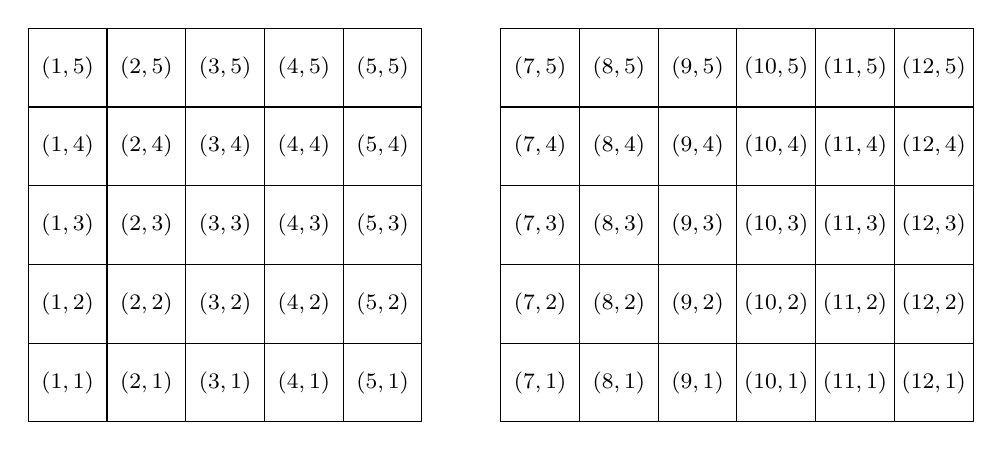
\begin{tikzpicture}
  \foreach \x in {1,2,...,5,7,8,...,12}
    \foreach \y in {1,...,5}
    {
      \draw (\x,\y) +(-.5,-.5) rectangle ++(.5,.5);
      \draw (\x,\y) node{\footnotesize $(\x,\y)$};
    }
\end{tikzpicture}
\end{lstlisting}
\end{minipage}
\end{center}
    \item \verb+[COMMIT]+ list your R/Sweave codes using \verb+lstlisting+
    \item \verb+[COMMIT]+ use the R/Sweave codes to compute
    \item \verb+[COMMIT]+ explain your computed numerical values 
    \item make sure to refer to your R code listing via \verb+\ref+ and to the
        computed values using \verb+\Sexpr+
    \item refer to  \cite{tikzManual2012-11-04} if necessary
\end{itemize}

\begin{figure}[h!]
    \centering
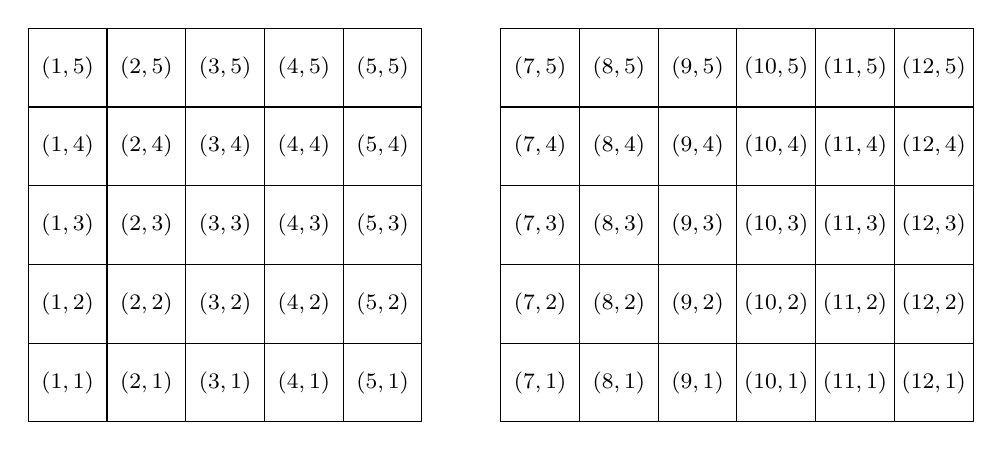
\begin{tikzpicture}
  \foreach \x in {1,2,...,5,7,8,...,12}
    \foreach \y in {1,...,5}
    {
      \draw (\x,\y) +(-.5,-.5) rectangle ++(.5,.5);
      \draw (\x,\y) node{\footnotesize $(\x,\y)$};
    }
\end{tikzpicture}
\caption{An extension of an example from the TikZ \& PGF manual \cite{tikzManual2012-11-04}}
\label{fig:examplefrommanual}
\end{figure}


\paragraph{Ex 4.2}
\begin{itemize}
    \item \verb+[COMMIT]+ list your R code using \verb+lstlisting+ 
    \item \verb+[COMMIT]+ demonstrate that your function is ``functioning'' by way of R/Sweave
\end{itemize}

\paragraph{Ex 4.3}
\begin{itemize}
    \item \verb+[COMMIT]+ list your R code using \verb+lstlisting+ 
    \item \verb+[COMMIT]+ load the data
        (\verb+require(MVA);data(gardenflowers)+) and compute using R/Sweave
    \item \verb+[COMMIT]+ include a plot of (relative) positions using R/Sweave
    \item \verb+[COMMIT]+ allocate at least a quarter page of \emph{text} explaining the result
\end{itemize}

\bibliographystyle{plain}
\nocite{*}
\bibliography{biblio}

\end{document}
